\documentclass[fullscreen=true, bookmarks=true, hyperref={pdfencoding=unicode}]{beamer}

\usepackage[utf8]{inputenc}                                % Кодировка
\usepackage[english,russian]{babel}                        % Переносы
\usepackage{xcolor}                                        % Работа с цветом
\usepackage{amsmath,amssymb,amsfonts}                      % Символы АМО
\usepackage{graphicx}                                      % Графика
\usepackage[labelsep=period]{caption}                      % Разделитель в подписях к рисункам и таблицам
\usepackage{hhline}                                        % Для верстки линий в таблицах
\usepackage[upright]{fourier}
\usepackage{verbatim}
\usepackage{tikz}                                          % Для простых рисунков в документе
\usetikzlibrary{matrix,arrows,decorations.pathmorphing,shapes.geometric,calc}
\usepackage{fancybox}                                      % Пакет для отрисовки рамок
\usepackage{verbatim}                                      % Для вставки кода в презентацию
\usepackage{xmpmulti}                                      % Для вставки gif в презентацию
\usepackage{multirow}
\usepackage{mathdots}

\usetikzlibrary{arrows,snakes,backgrounds}                 % Для отрисовки стрелок

\graphicspath{{../images/}}                                % Путь до рисунков
\setbeamertemplate{caption}[numbered]                      % Включение нумерации рисунков

\definecolor{links}{HTML}{2A1B81}                          % blue for url links
\hypersetup{colorlinks,linkcolor=,urlcolor=links}          % nothing for others

\usetheme{Malmoe}
\usecolortheme{seahorse}

% l' unite
\newcommand{\myunit}{1 cm}
\tikzset{
    node style sp/.style={draw,circle,minimum size=\myunit},
    node style ge/.style={circle,minimum size=\myunit},
    arrow style mul/.style={draw,sloped,midway,fill=white},
    arrow style plus/.style={midway,sloped,fill=white},
}

% \setbeameroption{show notes}
\setbeameroption{hide notes}

\title{Lecture 2. Determinants}
\author{Aleks Avdiushenko}
\institute{Neapolis University Paphos}
\date{May 17, 2023}
\titlegraphic{
\includegraphics[keepaspectratio,width=0.25\textwidth]{nup_logo.png}}

\begin{document}
%\unitlength=2mm

% выводим заглавие
\begin{frame}
\transdissolve[duration=0.2]
\titlepage
\end{frame}


\begin{frame}{Matrix Determinant}
  \begin{itemize}
    \item A determinant of square matrix is a \textbf{oriented} volume (area) of the parallelotope, made up of its column vectors
    \pause
    \item The determinant of a matrix $A$ is denoted as $|A|$ or $\det(A)$
    \pause
    \item Determinants can be calculated recursively using the cofactor formula
  \end{itemize}
  \pause
  \begin{example}
    For a $2 \times 2$ matrix, the determinant is calculated as:
    \[
      \det(A) = |A| = \begin{vmatrix}
        a_{11} & a_{12} \\
        a_{21} & a_{22}
      \end{vmatrix} = a_{11}a_{22} - a_{12}a_{21}
    \]      
  \end{example}
\end{frame}


\begin{frame}
  \frametitle{2D: oriented area}

  \begin{center}
    \begin{tikzpicture}[scale=0.8]
      \coordinate (O) at (0,0);
      \coordinate (A) at (4,1);
      \coordinate (B) at (1,3);
      \coordinate (C) at ($(A) + (B)$);

      \draw[->, thick] (O) -- (A) node[midway, below] {$\vec{a}$};
      \draw[->, thick] (O) -- (B) node[midway, left] {$\vec{b}$};
      \draw[->, thick] (A) -- (C) node[midway, right] {$\vec{b}$};
      \draw[->, thick] (B) -- (C) node[midway, above] {$\vec{a}$};
      \draw[dashed] (O) -- (C);

      \fill (O) circle (2pt) node[anchor=north east] {$O$};
      \fill (A) circle (2pt) node[anchor=north west] {$A$};
      \fill (B) circle (2pt) node[anchor=south east] {$B$};
      \fill (C) circle (2pt) node[anchor=south west] {$C$};
    \end{tikzpicture}
  \end{center}
  \begin{itemize}
    \item The above figure shows a parallelogram formed by two vectors $\vec{a}$ and $\vec{b}$
    \item The area of the parallelogram can be calculated using the determinant of the matrix formed by these vectors
    \[
      \det \begin{bmatrix}
        a_{1} & b_{1} \\
        a_{2} & b_{2}
      \end{bmatrix}
    \]      
  \end{itemize}
\end{frame}


\begin{frame}
  \frametitle{Three approaches for determinant}
  \begin{center}
    \begin{tikzpicture}[scale=1.2]
      % Center node
      \node[draw, circle, minimum size=1cm] (center) at (0, 0) {$|A|$};

      % Approach nodes
      \node[draw, rectangle, rounded corners, minimum width=2cm, minimum height=1cm] (approach1) at (210:2.5) {1. Formula};
      \node[draw, rectangle, rounded corners, minimum width=2cm, minimum height=1cm] (approach3) at (270:2.5) {2. Multilinear skew-symmetric functions};
      \node[draw, rectangle, rounded corners, minimum width=2cm, minimum height=1cm] (approach2) at (330:2.5) {3. Matrix multiplication};

      % Arrows
      \draw[->, thick] (center) -- (approach1);
      \draw[->, thick] (center) -- (approach2);
      \draw[->, thick] (center) -- (approach3);
    \end{tikzpicture}
  \end{center}
\end{frame}


\begin{frame}{1. Determinant Formula Through Permutations}
  \begin{itemize}
    \item The determinant of an $n \times n$ matrix $A = (a_{ij})$ can be calculated using permutations
    \item The set of all permutations of the first $n$ natural numbers is denoted by $S_n$
    \pause
    \item For each permutation $\sigma \in S_n$, its signature is defined 
    as $\operatorname{sgn}(\sigma)$, which is $1$ if $\sigma$ 
    can be obtained by an even number of transpositions, and $-1$ otherwise
    \item The determinant of the matrix $A$ can be calculated as:
    \[
      \det(A) = \sum_{\sigma \in S_n} \operatorname{sgn}(\sigma) 
      \prod_{i=1}^n a_{i\sigma(i)}
    \]
    \pause
    \item This formula expresses the determinant as a sum of $n!$ terms, one for each permutation in $S_n$
    \item Although this method can be computationally expensive, 
    it provides insight into the properties of determinants 
    and their relation to permutations
  \end{itemize}
\end{frame}


\begin{frame}{2. Multilinear Skew-Symmetric Function}
  \begin{itemize}
    \item A function $f$ on an $n \times n$ matrix is called multilinear if it is linear in each row and column separately
    \item A function $g$ is called skew-symmetric if its sign changes when two rows or two columns are interchanged, i.e., $g(\dots, x_i, \dots, x_j, \dots) = -g(\dots, x_j, \dots, x_i, \dots)$        
  \end{itemize}

  \pause
  \begin{block}{Definition}
    The determinant of a matrix can be characterized as the 
    \textbf{unique} multilinear skew-symmetric function 
    such that $\det(E) = 1$, where $E$ is the identity matrix
  \end{block}
\end{frame}


\begin{frame}
    This characterization helps in proving various properties 
    of determinants, such as the determinant of a product 
    of matrices and the determinant of a transpose
  
  \begin{example}
    Let $A$ and $B$ be two $n \times n$ matrices, then the determinant 
    of their product is equal to the product of their determinants:
    \[
      \det(AB) = \det(A) \cdot \det(B)
    \]  
  \end{example}
  
  Similarly, for a given matrix $A$, the determinant of its transpose 
  is equal to the determinant of the original matrix:
    \[
      \det(A^T) = \det(A)
    \]
  And also the determinant of inverse matrix:
  \[
    \det(A^{-1}) = \det(A)^{-1}
  \]
\end{frame}


\begin{frame}
  \frametitle{3. Matrix multiplication}

  Function $\Phi: M_{n}(\mathbb{R}) \to \mathbb{R}$

  \begin{itemize}
    \item $\Phi(AB) = \Phi(A)\cdot \Phi(B)$
    \item $\Phi \begin{pmatrix}
      1 & & & \\
        & \ddots & & \\
        &  & 1 & \\
        &  &   & \lambda
    \end{pmatrix} = \lambda$
  \end{itemize}
\end{frame}


\begin{frame}{How does determinant change with Elementary Row Transformations?}
  \begin{itemize}
    \pause
    \item Elementary row transformations are operations performed on the rows of a matrix. There are three types:
      \begin{enumerate}
        \item Row switching: interchange two rows
        \item Row scaling: multiply a row by a nonzero constant
        \item Row addition: add a multiple of one row to another row
      \end{enumerate}
      \pause
      \item The determinant of a matrix changes as follows with each type of elementary row transformation:
      \begin{enumerate}
        \item Row switching: $\det(A') = -\det(A)$, where $A'$ is obtained by switching two rows of $A$
        \item Row scaling: $\det(A') = k\det(A)$, where $A'$ is obtained by multiplying a row of $A$ by a nonzero constant $k$
        \item Row addition: $\det(A') = \det(A)$, where $A'$ is obtained by adding a multiple of one row to another row in $A$
      \end{enumerate}
  \end{itemize}
\end{frame}


\begin{frame}
  \frametitle{Upper triangular matrix}
  $$\begin{vmatrix}
    a_{11} & \dots & * &  * \\
    0 & a_{22} & \dots &  * \\
    \vdots & \ddots & \ddots & \\
    0 & \dots & 0 & a_{nn}
  \end{vmatrix} = a_{11}\cdot a_{22}\cdot \hdots \cdot a_{nn}
  $$

  \vspace{1cm}
  \pause
  \begin{block}{Note}
    \[
      \det(\lambda A) = \lambda^n \det(A)
    \]      
  \end{block}
\end{frame}


\begin{frame}{Geometric intuition}
  \centering  
  \begin{tikzpicture}
    % Draw the axes
    \draw[->] (0, 0) -- (2, 0) node[right] {$x$};
    \draw[->] (0, 0) -- (0, 2) node[above] {$y$};
    
    % Draw the unit square
    \draw[fill=blue!20] (0, 0) -- (1, 0) -- (1, 1) -- (0, 1) -- cycle;
    % Draw the parallelogram
    \draw (0, 0) -- (1.5, 1) -- (2.5, 1) -- (1, 0) -- cycle;
    
    % Add labels
    \node at (0.6, 1.5) {
      $\begin{bmatrix}
        1 & 0 \\
        0 & 1 
      \end{bmatrix}$
    };
    \node at (2.25, 1.5) {
      $\begin{bmatrix}
        1 & \lambda \\
        0 & 1 
      \end{bmatrix}$
    };
  \end{tikzpicture}
\end{frame}


\begin{frame}{Examples}
  \begin{itemize}
    \pause
    \item $\det \begin{vmatrix}
      1 & 2 \\
      3 & 4 
    \end{vmatrix} = -2$
    \pause
    \item $\det \begin{vmatrix}
      1 & 2 & 3 \\
      4 & 5 & 6 \\
      7 & 8 & 9
    \end{vmatrix} = 0$  
    \pause
    \item $\det \begin{vmatrix}
      x & 1 & 1 \\
      1 & \ddots & 1 \\
      1 & 1 & x
    \end{vmatrix} = ?$  
  \end{itemize}
\end{frame}


\begin{frame}{Solution}
  \begin{align*}
    \det \begin{vmatrix}
      x & 1 & 1 \\
      1 & \ddots & 1 \\
      1 & 1 & x
    \end{vmatrix} &= 
        \det \begin{vmatrix}
      x+n-1 & \dots & x+n-1 \\
      1 & \ddots & 1 \\
      1 & 1 & x
    \end{vmatrix} = \\
    (x+n-1) \det \begin{vmatrix}
      1 & 1 & 1 \\
      1 & \ddots & 1 \\
      1 & 1 & x
    \end{vmatrix} &= 
    (x+n-1) \det \begin{vmatrix}
      1 & 1 & 1 \\
      0 & \ddots & 1 \\
      0 & 0 & x-1
    \end{vmatrix} = \\
    &= (x+n-1) (x-1)^{n-1}
  \end{align*}
\end{frame}


\begin{frame}{Task 1}
  $$\det \begin{vmatrix}
    x & \dots & x & x \\
      &   1 &   x &  x \\
    1 & \iddots  & 1   &  \vdots \\
    x & 1 &   &  x
  \end{vmatrix}\ =\ ?$$
\end{frame}


\begin{frame}{Block formula for determinant N1}
  \newcommand{\sidelen}{3cm}
  \newcommand{\shift}{0.25cm}
  \centering
  \begin{tikzpicture}
    \draw (0, 0) -- node [left] {$\det$} ++(0, \sidelen) -- ++(\sidelen, 0) 
    -- ++(0, -\sidelen) -- ++(-\sidelen, 0);
    \draw (0, \sidelen/2) -- ++(\sidelen, 0);
    \draw (\sidelen/2, 0) -- ++(0, \sidelen);
    \coordinate [label={$A$}] () at (\sidelen/4, 3*\sidelen/4-\shift);
    \coordinate [label={$B$}] () at (3*\sidelen/4, 3*\sidelen/4-\shift);
    \coordinate [label={$0$}] () at (\sidelen/4, \sidelen/4-\shift);
    \coordinate [label={$D$}] () at (3*\sidelen/4, \sidelen/4-\shift);

    \coordinate [label={$= \det A \det D$}] () at (5*\sidelen/4+2*\shift, \sidelen/2-\shift);
  \end{tikzpicture}
\end{frame}


\begin{frame}{Van der Monde Determinant}
  \begin{itemize}
    \item The Van der Monde determinant is a specific kind of determinant of a square matrix
    \item It has the form:
      \[
      \begin{vmatrix}
        1      & 1      & \cdots & 1      \\
        x_1    & x_2    & \cdots & x_n    \\
        x_1^2  & x_2^2  & \cdots & x_n^2  \\
        \vdots & \vdots & \ddots & \vdots \\
        x_1^{n-1} & x_2^{n-1} & \cdots & x_n^{n-1}
      \end{vmatrix}
      \]
    \pause
    \item The determinant of this matrix can be computed as:
      \[
      \prod_{1 \leq i < j \leq n} (x_j - x_i)
      \]
  \end{itemize}
\end{frame}


\begin{frame}{Solution}
  \begin{align*}
    \det 
    \begin{vmatrix}
      1      & 1      & 1 & 1  \\
      x_1    & x_2    & x_3 & x_4    \\
      x_1^2  & x_2^2  & x_3^2 & x_4^2  \\
      x_1^{3} & x_2^{3} & x_3^{3} & x_4^{3}
    \end{vmatrix}  
    = \\ = \det 
    \begin{vmatrix}
      1      & 1      & 1 & 1      \\
      0    & x_2 - x_1 & x_3 - x_1 & x_4 - x_1 \\
      0  & x_2^2 - x_1x_2  & x_3^2 - x_1x_3 & x_4^2 - x_1x_4  \\
      0 & x_2^{3} - x_1x_2^2 & x_3^{3} - x_1x_3^2 & x_4^{3}- x_1x_4^2
    \end{vmatrix} = \\ =
    (x_2 - x_1) (x_3 - x_1) (x_4 - x_1) \det 
    \begin{vmatrix}
      1      & 1      & 1 \\
      x_2    & x_3    & x_4 \\
      x_2^2  & x_3^2 & x_4^2 
    \end{vmatrix}  
  \end{align*}
\end{frame}


\begin{frame}{Polynomial Interpolation}
  \begin{columns}
      \begin{column}{.3\paperwidth}
        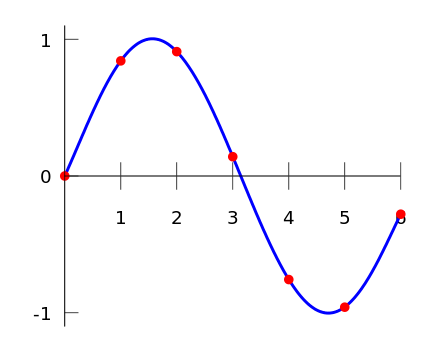
\includegraphics[keepaspectratio, width=.3\paperwidth]{440px-Interpolation_example_polynomial.png}
      \end{column}
      \begin{column}{.7\paperwidth}
        \begin{itemize}
        \item Polynomial interpolation is a method of fitting 
        a polynomial function to a set of n points $(x_i, y_i)$, $i = 1, 2, \dots, n$
        \item The goal is to find a polynomial $P(x)$ of degree less than $n$, 
        such that $P(x_i) = y_i$ for all $i = 1, 2, \dots, n$
        \item The polynomial can be written as:
          \[
          P(x) = a_0 + a_1x + a_2x^2 + \cdots + a_{n-1}x^{n-1}
          \]
      \end{itemize}          
    \end{column}
  \end{columns}
\end{frame}


\begin{frame}{SLE for interpolation}
  By solving a system of linear equations, 
  we can find the coefficients $a_i$ that make the polynomial 
  interpolate the given points
\[
  \begin{bmatrix}
    1      & x_1    & x_1^2  & \cdots & x_1^{n-1} \\
    1      & x_2    & x_2^2  & \cdots & x_2^{n-1} \\
    \vdots & \vdots & \vdots & \ddots & \vdots \\
    1      & x_n    & x_n^2  & \cdots & x_n^{n-1}
  \end{bmatrix}
  \begin{bmatrix}
    a_0 \\
    a_1 \\
    \vdots \\
    a_{n-1}
  \end{bmatrix} =
  \begin{bmatrix}
    y_1 \\
    y_2 \\
    \vdots \\
    y_n
  \end{bmatrix}
\]
\pause
\begin{block}{Note 1}
    $A$ is invertible $\iff \det(A) \neq 0$ (we will discuss it later)
\end{block}
\pause
\begin{block}{Note 2}
  We have one-to-one correspondence between

  coefficients $a_0, \hdots, a_{n-1}$ and point values $(x_1, y_1), \hdots, (x_n, y_n)$
\end{block}
\end{frame}


\begin{frame}{Cofactor Formula for Determinants}
  \begin{itemize}
    \item The cofactor formula is a recursive method for calculating the determinant of a square matrix
    \item For an $n \times n$ matrix $A$, its determinant can be calculated using the formula (first row decomposition):
      \[
      \det(A) = \sum_{j=1}^n a_{1j} C_{1j},
      \]
      where $a_{1j}$ is the element in the first row and $j$-th column, and $C_{1j}$ is the cofactor of that element
    \pause
    \item The cofactor $C_{ij}$ is defined as:
      \[
      C_{ij} = (-1)^{i+j} \det(M_{ij}),
      \]
      where $M_{ij}$ is the $(n-1) x (n-1)$ matrix obtained by removing the i-th row and j-th column from $A$
    \item The cofactor formula can be applied recursively until a $2 \times 2$ or 
    $1 \times 1$ matrix is reached, at which point the determinant 
    can be calculated directly
  \end{itemize}
\end{frame}


\begin{frame}{Explicit formula for inverse matrix}
  \begin{itemize}
    \item Let A be an $n \times n$ invertible matrix. The inverse of $A$, 
    denoted as $A^{-1}$, is also an $n \times n$ matrix
    \item The coefficients of the inverse matrix can be found using the formula:
      \[
      (A^{-1})_{ij} = \frac{C_{ji}}{\det(A)},
      \]
      where $C_{ji}$ is the cofactor of the element in the $j$-th row 
      and $i$-th column of $A$, and $\det(A)$ is the determinant of $A$
  \end{itemize}

  \pause
  \begin{block}{Note}
    The indices $i$ and $j$ are swapped in the cofactor, 
    which means that the cofactor matrix is transposed
  \end{block}

\end{frame}


\begin{frame}{Cramer's Formulas}
  \begin{itemize}
    \item Cramer's formulas provide a method for 
    solving a system of linear equations using determinants
    \item Let $A$ be an $n \times n$ matrix, and 
    let $\textbf{b}$ be an $n \times 1$ column vector. 
    Consider the linear system $A\textbf{x} = \textbf{b}$
    \item If $\det(A) \neq 0$, the system has a unique solution given by Cramer's formulas:
      \[
      x_i = \frac{\det(A_i)}{\det(A)}, \quad i = 1, 2, \ldots, n,
      \]
      where $A_i$ is the matrix obtained by replacing the $i$-th column of $A$ 
      with the vector $\textbf{b}$
  \end{itemize}

  \pause
  \begin{block}{Note}
    \small
    Cramer's formulas can be computationally expensive, as they require 
    calculating $n + 1$ determinants for an $n \times n$ system
    
    However, they can be useful for understanding 
    the geometry of linear systems and for solving small systems 
    or systems with a specific structure
  \end{block}
\end{frame}


\begin{frame}{Block formula for determinant N2}
  \newcommand{\sidelen}{3cm}
  \newcommand{\shift}{0.25cm}
  \centering
  $\det A \neq 0$
  
  \begin{tikzpicture}
    \draw (0, 0) -- node [left] {$\det$} ++(0, \sidelen) 
    -- ++(\sidelen, 0)
    -- ++(0, -\sidelen) -- ++(-\sidelen, 0);
    \draw (0, \sidelen/2) -- ++(\sidelen, 0);
    \draw (\sidelen/2, 0) -- ++(0, \sidelen);
    \coordinate [label={$A$}] () at (\sidelen/4, 3*\sidelen/4-\shift);
    \coordinate [label={$m$}] () at (\sidelen/4, 4*\sidelen/4);
    \coordinate [label={$m$}] () at (-\shift, 3*\sidelen/4-\shift);
    
    \coordinate [label={$B$}] () at (3*\sidelen/4, 3*\sidelen/4-\shift);
    \coordinate [label={$C$}] () at (\sidelen/4, \sidelen/4-\shift);
    
    \coordinate [label={$D$}] () at (3*\sidelen/4, \sidelen/4-\shift);
    \coordinate [label={$n$}] () at (3*\sidelen/4, -1.6*\shift);
    \coordinate [label={$n$}] () at (4*\sidelen/4+\shift, \sidelen/4-\shift);

    \coordinate [label={$= \det A \det (D - CA^{-1}B)$}] () at 
    (6*\sidelen/4+3*\shift, \sidelen/2-1.5*\shift);
  \end{tikzpicture}
\end{frame}


\begin{frame}{How to prove it?}
  Blocks as «numbers»:
  \vspace{1cm}
  
  \newcommand{\sidelen}{3cm}
  \newcommand{\shift}{0.25cm}
  \begin{tikzpicture}
    \draw (0, 0) -- ++ (0, \sidelen) -- ++  (\sidelen, 0) 
    -- ++ (0, -\sidelen) -- ++ (-\sidelen, 0);
    \draw (0, \sidelen/2) -- ++ (\sidelen, 0);
    \draw (\sidelen/2, 0) -- ++ (0, \sidelen);
    \coordinate [label={$A$}] () at (\sidelen/4, 3*\sidelen/4-\shift);
    \coordinate [label={$B$}] () at (3*\sidelen/4, 3*\sidelen/4-\shift);
    \coordinate [label={$C$}] () at (\sidelen/4, \sidelen/4-\shift);
    \coordinate [label={$D$}] () at (3*\sidelen/4, \sidelen/4-\shift);

    \draw (\sidelen+2*\shift, 0) -- node [left] {$=$} ++ (0, \sidelen) 
    -- ++  (\sidelen, 0) 
    -- ++ (0, -\sidelen) -- ++ (-\sidelen, 0);
    \draw (\sidelen+2*\shift, \sidelen/2) -- ++ (\sidelen, 0);
    \draw (3*\sidelen/2+2*\shift, 0) -- ++ (0, \sidelen);
    \coordinate [label={$A$}] () at (5*\sidelen/4+2*\shift, 3*\sidelen/4-\shift);
    \coordinate [label={$0$}] () at (7*\sidelen/4+2*\shift, 3*\sidelen/4-\shift);
    \coordinate [label={$0$}] () at (5*\sidelen/4+2*\shift, \sidelen/4-\shift);
    \coordinate [label={$E$}] () at (7*\sidelen/4+2*\shift, \sidelen/4-\shift);

    \draw (2*\sidelen+3*\shift, 0) -- ++ (0, \sidelen) -- ++  (1.5*\sidelen, 0) 
    -- ++ (0, -\sidelen) -- ++ (-1.5*\sidelen, 0);
    \draw (2*\sidelen+3*\shift, \sidelen/2) -- ++ (1.5*\sidelen, 0);
    \draw (11*\sidelen/4+3*\shift, 0) -- ++ (0, \sidelen);
    \coordinate [label={$E$}] () at (10*\sidelen/4+1.5*\shift, 3*\sidelen/4-\shift);
    \coordinate [label={$A^{-1}B$}] () at (13*\sidelen/4+1.5*\shift, 3*\sidelen/4-\shift);
    \coordinate [label={$C$}] () at (10*\sidelen/4+1.5*\shift, \sidelen/4-\shift);
    \coordinate [label={$D$}] () at (13*\sidelen/4+1.5*\shift, \sidelen/4-\shift);
  \end{tikzpicture}
\end{frame}


\begin{frame}{And also}
  \newcommand{\sidelen}{3cm}
  \newcommand{\shift}{0.25cm}
  \centering
  For the appropriate dimensions and $AC = CA$
  \vspace{1cm}
  
  \begin{tikzpicture}
    \draw (0, 0) -- node [left] {$\det$} ++(0, \sidelen) 
    -- ++(\sidelen, 0)
    -- ++(0, -\sidelen) -- ++(-\sidelen, 0);
    \draw (0, \sidelen/2) -- ++(\sidelen, 0);
    \draw (\sidelen/2, 0) -- ++(0, \sidelen);
    \coordinate [label={$A$}] () at (\sidelen/4, 3*\sidelen/4-\shift);
    
    \coordinate [label={$B$}] () at (3*\sidelen/4, 3*\sidelen/4-\shift);
    \coordinate [label={$C$}] () at (\sidelen/4, \sidelen/4-\shift);
    
    \coordinate [label={$D$}] () at (3*\sidelen/4, \sidelen/4-\shift);

    \coordinate [label={$= \det (AD - CB)$}] () at 
    (6*\sidelen/4, \sidelen/2-1.5*\shift);
  \end{tikzpicture}

  \begin{block}{Note}
    It can be proved by the continuation by continuity method: $A_\lambda = A - \lambda E$
  \end{block}
\end{frame}


\begin{frame}{Matrix Characteristic Polynomial}
  \begin{itemize}
    \item For an $n \times n$ matrix $A$, the characteristic polynomial 
    $\chi_A(\lambda)$ is defined as:
      \[
        \chi_A(\lambda) = \det(\lambda E - A),
      \]
      where $\lambda$ is a scalar variable and $E$ is the $n \times n$ identity matrix
    \item The characteristic polynomial is of degree $n$, 
    and its roots are the eigenvalues of the matrix $A$
    \item The characteristic equation is given by:
      \[
        \chi_A(\lambda) = 0,
      \]
      which is an algebraic equation that can be used to find the eigenvalues of $A$
    \item The characteristic polynomial and its properties 
    play a crucial role in linear algebra, 
    especially in the study of matrix diagonalization, 
    eigenvectors, and matrix functions
  \end{itemize}
\end{frame}


\begin{frame}{Characteristic Polynomial Properties}
  \[
    \chi_A(\lambda) = \det(\lambda E - A) = 
    \lambda^n + a_{n-1}\lambda^{n-1} + \hdots + a_0
  \]
  \begin{itemize}
    \item $a_0 = (-1)^n \det A$
    \item $a_{n-1} = -\mathrm{tr} A$
    \item $\lambda \in \mathrm{Spec}A \iff \lambda E - A \text{ is irreversible}
    \iff \det(\lambda E - A) = 0 \iff \lambda \text{ is root of } \chi_A$
  \end{itemize}
\end{frame}


\begin{frame}{Cayley--Hamilton Theorem}
  \begin{itemize}
    \item The Cayley--Hamilton theorem is a fundamental result 
    in matrix theory that states that every square matrix satisfies 
    its own characteristic equation
    \pause
    \item So let $A$ be an $n \times n$ matrix 
    with the characteristic polynomial $\chi_A(\lambda)$. 
    Then, the Cayley--Hamilton theorem states that:
      \[
        \chi_A(A) = 0,
      \]
      where 0 is the $n \times n$ zero matrix
    \pause
    \item The theorem provides a powerful tool for finding 
    matrix inverses, matrix powers, and solving systems of 
    linear differential equations
    \item It also has important implications for the study 
    of matrix functions, matrix diagonalization, and 
    the minimal polynomial of a matrix
  \end{itemize}

  \pause
  \begin{block}{Note}
    \small This is a non-trivial result given by the annihilating polynomial 
    of degree $n$, and in the general case it is impossible 
    to reduce this degree.
  \end{block}
\end{frame}


\begin{frame}
  \begin{example}
    $A=E$

    $$f_{\min} (x) = x - 1$$

    $$ \chi_A(x) = (x-1)^n$$
  \end{example}
\end{frame}


\begin{frame}{Task 2}
  $d_n = \det \begin{vmatrix}
    a & b & 0 & 0 \\
    c & \ddots & \ddots & 0 \\
    0 & \ddots & \ddots & b \\
    0 & 0 & c & a 
  \end{vmatrix} = ?$  

  \pause
  \begin{align*}
    d_n &= a \cdot d_{n-1} - bc \cdot d_{n-2} \\
    d_1 &= a \\
    d_2 &= a^2-bc
  \end{align*}
  
  \begin{columns}
    \begin{column}{0.5\paperwidth}
      \pause
      $$\begin{pmatrix}
        d_n \\
        d_{n-1}
      \end{pmatrix} = 
      \begin{pmatrix}
        a & -bc \\
        1 & 0
      \end{pmatrix}  
      \begin{pmatrix}
        d_{n-1} \\
        d_{n-2}
      \end{pmatrix}$$
    
      $$ x_n = A x_{n-1} = A^2 x_{n-2} = \hdots = A^{n-2} x_2 $$          
    \end{column}
    \begin{column}{0.5\paperwidth}
      \pause
      $$d_n = \lambda^n \Rightarrow \lambda^n = a \lambda^{n-1} - bc \lambda^{n-2}$$
      $$\lambda^2 - a \lambda + bc = 0 $$
      \begin{align*} 
        \text{If }\lambda_1 \neq \lambda_2 \text{ are roots } \Rightarrow d_n = c_1\lambda_1^n + c_2\lambda_2^n \\
        \text{If }\lambda_1 = \lambda_2 \Rightarrow d_n = (c_1 + c_2n)\lambda_1^n 
      \end{align*} 
    \end{column}
  \end{columns}
\end{frame}


\begin{frame}{Task 3}
  Let matrix $A \in M_n(\mathbb{R})$. Find $\det \widehat{A}$,
  where $\widehat{A} = (C_{ij})^T$

  \pause
  \begin{block}{Solution}
    \pause
    $$\det \widehat{A} = \det A^{n-1}$$
  
    \pause
    $$A\widehat{A} = \widehat{A} A = \det A \cdot E $$
    $$\det A \det\widehat{A} = \det (\det A \cdot E ) = \det A^n$$
    If $\det A \neq 0$, then we've solved. 

    Otherwise, $\widehat{A} A = 0 \Rightarrow \exists$ column 
    $A_i \neq 0: \widehat{A} A_i = 0 \Rightarrow \widehat{A}$ is irreversible
    $$ \Rightarrow \det \widehat{A} = 0$$
  \end{block}
\end{frame}


\end{document}